\documentclass{letter}
\usepackage[margin=0.75in]{geometry}
\usepackage{amsmath}
\usepackage{amssymb}
\usepackage{enumerate}
\usepackage{tikz}
\usepackage{pgfplots}
\pgfplotsset{compat=1.8}

\pgfplotsset{vasymptote/.style={
		before end axis/.append code={
			\draw[densely dashed] ({rel axis cs:0,0} -| {axis cs:#1,0})
			-- ({rel axis cs:0,1} -| {axis cs:#1,0});
		}
	}}

\begin{document}
	\begin{center}
		\LARGE Math137 - November 11, 2015\\
		\large Curve Sketching - Applied Max/Min Problems
	\end{center}
	\vspace{0.25 in}
	\underline{\textbf{Example}}
	
	Sketch the following function: $y = (\frac{\ln(x)}{x})^2$
	
	\begin{minipage}[t]{0.5\textwidth}
		\begin{enumerate}[i)]
			\item \textbf{X Intercepts:}\\
			$\ln(x) = 0$\\
			$x = 1$\\\\
			
			\setcounter{enumi}{2}
			\item \textbf{Vertical Asymptotes:}\\
			$x=0$
			On the positive side of 0, the goes to infinity. On the left side, the function is undefined.
			\\\\\setcounter{enumi}{4}
			\item \textbf{Critical Values:}
			\begin{flalign*}
				f(x) &= (\frac{\ln x}{x})^2&\\
				f'(x) &= 2(\frac{\ln x}{x})(\frac{(\frac{1}{x}(x)-\ln x}{x^2})\\
				&= \frac{(2)(\ln x)(1 - \ln x)}{x^3}\\
			\end{flalign*}
			$\therefore$ Critical values are $1, e, 0$.\\
			\setcounter{enumi}{6}
			\item \textbf{Concavity}
			\begin{flalign*}
				f'(x) &= \frac{2 \ln x - 2(\ln x)^2}{x^3}&\\
				f''(x) &= \frac{(\frac{2}{x} - \frac{4\ln x}{x})x^3 - (2 \ln x - 2(\ln x)^2)3x^2}{x^6}\\
				&= \frac{2x^2 - 4(\ln x)(x^2) - (2\ln x - 2(\ln x)^2)(3x^2)}{x^6}\\
				&= \frac{2 - 4\ln x - 6\ln x + 6(\ln x)^2}{x^4}\\
				&= \frac{2(3(\ln x)^2 - 5\ln x + 1)}{x^4}\\
				\ln x &= \frac{5 +- \sqrt{25 - 4(3)(1)}}{6}\\
				&= \frac{5 +- \sqrt{13}}{6}\\
				x &\approx e^{1.43}, e^{0.23}\\
				&\approx 4.18, 1.26
			\end{flalign*}
		\end{enumerate}
	\end{minipage}
	\begin{minipage}[t]{0.5\textwidth}
		\begin{enumerate}[i)]
			\setcounter{enumi}{1}
			\item \textbf{Y Intercept:}\\
			$y = (\frac{\ln(0)}{0})^2$\\
			This function does not exist at 0, so there is no y intercept.\\
			\setcounter{enumi}{3}
			\item \textbf{Horizontal End Behavior:}\\
			As x gets big positively, $x$ overpowers $\ln(x)$, so the function tends to 0.\\
			As x gets big negatively, The function does not exist.\\
			\setcounter{enumi}{5}
			\item \textbf{Increasing/Decreasing Intervals}\\
			
			\begin{tabular}{c|c|c|c|c}
				&$x<0$&$0<x<1$&$1<x<e$&$x>e$\\
				\hline
				$2(\ln x)(1 - \ln x)$&dne&-&+&-\\
				$x^3$&-&+&+&+\\
				$f'$&dne&-&+&-\\
				$f$&dne&Dec.&Inc.&Dec.\\
			\end{tabular}\\
			\\\;\\
			\begin{minipage}[t]{0.45\textwidth}
				$f(1) = (\frac{\ln 1}{1})^2$\\
				$f(1) = 0$\\
				So, min at (1, 0)\\
			\end{minipage}
			\begin{minipage}[t]{0.45\textwidth}
				$f(e) = (\frac{\ln e}{e})^2$\\
				$f(e) = \frac{1}{e^2}$\\
				So, max at $(e, \frac{1}{e^2})$
			\end{minipage}
			\setcounter{enumi}{7}
			\item \textbf{Intervals of Concavity and POIs}	\\
			\begin{tabular}{c|c|c|c|c}
				&$x<0$&$0<x<1.26$&$1.26 < x < 4.18$&$x > 4.18$\\
				Num.&dne&+&-&+\\
				Denom.&+&+&+&+\\
				$f''$&dne&+&-&+\\
				$f$&dne&Conc. Up&Conc. Down&Conc.Up\\
			\end{tabular}
			\\\\\\
			The function exists at $x=1.26, 4.18$, and concavity changes at these values so they are points of inflection.\\
			\begin{center}$y = (\frac{\ln x}{x})^2$\end{center}
			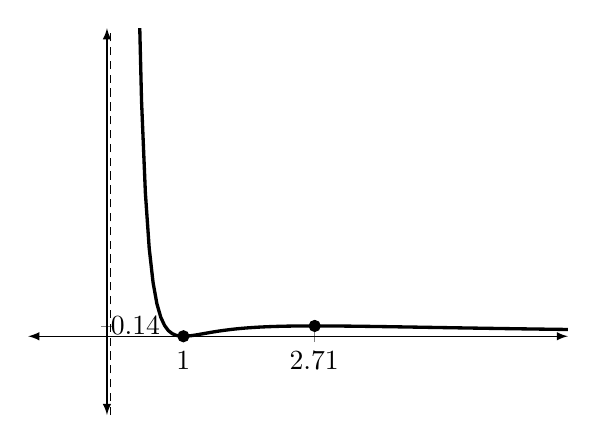
\begin{tikzpicture}
			\begin{axis}[
			axis equal image,
			axis lines=middle,
			xmin=0,xmax=5,
			ymin=0,ymax=3,
			enlargelimits={abs=1cm},
			axis line style={latex-latex},
			yticklabel style={anchor=west},
			ytick={0.135},
			xtick={1,  2.71},
			vasymptote=0.05,
			]
			% This doesn't clip to y=-10:10 nicely
			% because there are too few samples near the asymptote:
			\addplot[very thick, black, domain=0:10,samples=200, restrict y to domain=0:100]
			{((ln(x))/(x))^2};
			\addplot[only marks] table {
			1 0
			2.718 0.135	
			};
			
			
			\end{axis}
			\end{tikzpicture}\\
		\end{enumerate}
	\end{minipage}
	\pagebreak\\
	\underline{\textbf{Applied Max/Min Problems, Optimization}}
	
	\textbf{Examples:}
	 \begin{enumerate}[i) ] \item Find the point on the parabola $y=x^2$ which is closest to the point $(6, 3)$.
	
	\begin{center}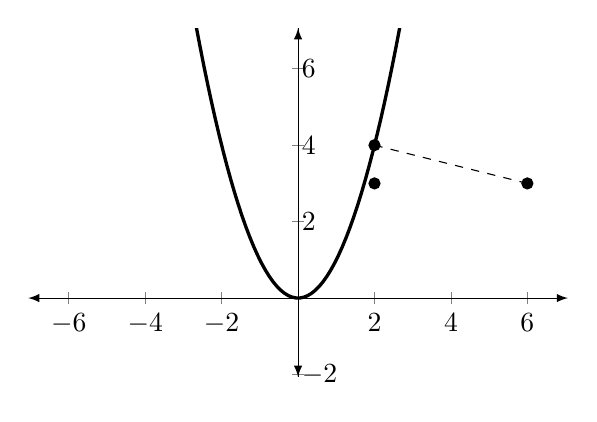
\begin{tikzpicture}
		\coordinate (a) at (6,3);
		\coordinate (b) at (2,4);
		\begin{axis}[
		axis equal image,
		axis lines=middle,
		xmin=-5,xmax=5,
		ymin=0,ymax=5,
		enlargelimits={abs=1cm},
		axis line style={latex-latex},
		yticklabel style={anchor=west},
		ytick={},
		xtick={},
		vasymptote=0,
		]
		% This doesn't clip to y=-10:10 nicely
		% because there are too few samples near the asymptote:
		\addplot[very thick, black, domain=-10:10,samples=200, restrict y to domain=0:100]
		{x^2};
		\addplot[dashed, black, domain=2:6,samples=200, restrict y to domain=0:100]
		{((-1/4)*(x-6) + 3};
		\addplot[only marks] table {
			6 3
			2 4
			2 3
		};
		\end{axis}
	\end{tikzpicture}\end{center}
	We want to minimize distance $d$, the length of the line segment from the nearest point on the parabola to $(6, 3)$. If we were to choose some point $P$ on our parabola, we could create a triangle connecting $P$, $(6, 3)$, and a point consisting of the x value of $P$ and the y value of $(6, 3)$. That's confusing, so look at the diagram above.\\
	
	$d^2 = (x-6)^2 +(x-3)^2$\\
	
	\textbf{Critical Points:}
	\begin{flalign*}
		\frac{d d^2}{dx} &= 2(x-6) + 4x(x^2 - 3)&\\
		&= 2(2x^3 -5x-6)\\
		&= (x-2)(2x^2+4x+3)\\
	\end{flalign*}
	$2x^2+4x+3=0$ has no real solutions, so the only critical value is $x=2$. If we check, we see the derivative is negative before $x=2$ and positive after $x=2$, so $x=2$ is the minimum.\\
	$y = (2)^2$\\
	$y = 4$\\
	
	$\therefore$ the closest point on the function $y=x^2$ to the point $6, 3)$\\
	
	\item A rain gutter is to be constructed from a metal sheet of width 30cm by bending $\frac{1}{3}$ of the sheet up at both sides through an angle $\theta$. How should $\theta$ be chosen to maximize the amount of water contained?
	
	I have no idea how to illustrate this, so I'll explain it. We have a 30cm flat metal sheet. We want to bend up the 10cm at both ends to maximize the amount of water contained. Bending up the 10 cm at both ends creates a trapazoid with theta representing the angle between the ground and the sheet. We want to find theta such that the area of our trapezoid is maximized.\\
	
	$A(\theta) = (10h) + 10h\cos(\theta)$\\
	As $h = 10\sin(\theta)$, \\
	$A(\theta) = 100\sin(\theta)(1+\cos(\theta))$\\
	$\frac{dA}{d\theta} = 100\cos(\theta)(1+\cos(\theta)) - 100\sin^2(\theta)$\\
	
	Set derivative equal to 0 for Critical Values.\\
	
	$0 = 100(\cos^2\theta - \sin^2\theta + \cos\theta)$\\
	$0 = 2\cos^2\theta + \cos\theta - 1$
	$0 = (2\cos\theta - 1)(\cos\theta + 1)$\\
	
	So, $\cos\theta = \frac{1}{2}$ or $-1$\\
	-1 is out of our interval, so $\frac{\pi}{3}$ is our theta that maximizes area.
	\end{enumerate}
\end{document}